% fancytikzposter.tex, version 2.1
% Original template created by Elena Botoeva [botoeva@inf.unibz.it], June 2012
% 
% This file is distributed under the Creative Commons Attribution-NonCommercial 2.0
% Generic (CC BY-NC 2.0) license
% http://creativecommons.org/licenses/by-nc/2.0/ 


\documentclass{a0poster}

\usepackage{fancytikzposter} 
\usepackage{fancySettings} 
\usepackage{mystyle}

%%%%%%%%%%%%%%%%%%%%%%%%%%%%%%%%%%%%%%%%%%%%%%%%%%%%%%%%%%%%%%%%%%%%%%%%%%%%%%%%%%%%%%%%%%%%%%%%%%%%%%%%%%%%%%%%%%%%%%%%%%%%%%%%%%%%%%%%%%%%%%%%%%%%%%%%%%%%%%%%%%%%%%%%%%%%%%%%%%%%%%%%%%%%%%

\title{Parallel Tempering \qquad }
\author{ \udot{Mateusz Łącki} \and Błażej Miasojedow\\
  Wydział Matematyki, Informatyki i Mechaniki\\ University of Warsaw, Poland\\
  \texttt{mateusz.lacki@biol.uw.edu.pl}\\
  \texttt{B.Miasojedow@mimuw.edu.pl} 
}

\usetemplate{1}

\begin{document}

\ClearShipoutPicture
\AddToShipoutPicture{\BackgroundPicture}

\noindent % to have the picture right in the center
\begin{tikzpicture}
  \initializesizeandshifts
  % \setxshift{15}
  % \setyshift{2}


  %% the title block, #1 - shift, the default value is (0,0), #2 - width, #3 - scale
  %% the alias of the title block is `title', so we can refer to its boundaries later
\ifthenelse{\equal{\template}{1}}{ 
  \titleblock{47}{1}
}{
  \titleblock{47}{1.5}
}


  %% #1 - anchor relative to the title block, #2 - shift, #3 - width, #3 - file name
\addlogo[south west]{(2,1.5)}{8cm}{img/logoUniversityOfWarsaw.png}
% \addlogo[south east]{(-2,1.5)}{16cm}{img/logoMimuw.png}


%%%%%%%%%%%%%%%%%%%%%%%%%%%%%%%%%%%%%%%%%%%%%%%%%%%%%%%%%%%%%%%%%%%%%%%%%%%%%%%%%%%%%%%%%%%%%%%%%%%%%%%%%%%%%%%%%%%%%%%%%%%%%%%%%%%%%%%%%%%%%%%%%%%%%%%%%%%%%%%%%%%%%%%%%%%%%%%%%%%%%%%%%%%%%%


\blocknode{Bayesian Inference in Bioinformatics}{
  % \coloredbox{colorthree!50!}
  % {\centering Bayesian Inference}
    \bi
      \item{ Suppose we can measure some quantity $y$. Assume, that parameter $\alpha$   describes $y$'s distribution}
      \bi
        \item{ let both be random and their joint density $g(y,\alpha)$ factorise so that
          $ g(y,\alpha) = h(y| \alpha) f( \alpha )$, where $f$ is {\it a priori} distribution on the parameter
        }
        \item{ $f$ might result from an underlying physical theory}
      \ei
      \item{ Real sample points $\mathfrak{y} = [ y_1, \dots, y_\mm ]$ are observed}
      \item{ The {\it a posteriori} distribution of $\alpha$ given the sample $\mathfrak{y}$, $f(\alpha| \mathfrak{y})$, describes how our knowledge about the studied quantity $x$ is influenced by empirical evidence collected in $\mathfrak{y}$}
      \bi
        \item{Obtain it via the Bayes Formula
          $$ 
            f(\alpha| \mathfrak{y}) = 
            \frac{ 
              h(y_1|\alpha) \dots h(y_\mm|\alpha) f(\alpha)
            }{
              \int h(y_1|\beta)\dots 
            h(y_\mm|\beta) f(\beta) \mathrm{d}\,\beta} $$
        }
      \ei
    \ei
  \coloredbox{colorthree!50!}
  {\centering Applications}
  \bi
    \item{ Hierarchical modelling for identification of co-expression patterns in microarray
data by cluster analysis \citep{Medvedovic, STING2010} }

    \item{ Assessing the importance of explanatory variables \citep{STING2010} }

    \item{ Model Selection }
  \ei
  \coloredbox{colorthree!50!}{\centering \mcmc}
  \bi
    % \item{ Closed formulas exist only in very restricted case of considering conjugate priors }

    \item{ \mcmc\, algorithms are used to simulate samples out of analytically untractable posterior distributions }
    \bi
      \item{ Most popular algorithm: \GreenMetropolisHastings\, \citep{Geyer}}
      \item{ Generates a sequence of points that are thought of as being an instantiation of a Markov Chain, $X \equiv \{ X^{[k]}\}_{k = 0}^\infty$  }
      \item{ Each point $X^{[k]}$ is generated by accepting or rejecting at random a step proposal given the chains last position $X^{[k-1]}$ }
      \item{ Approximates, thanks to Ergodic Theory, integrals 
        $$\expect g(X) = \int_\Omega g(x) \pi(x)\mathrm{d}\,x \approx \frac{1}{\nn}\sum_{i = 1}^\nn g(X^{[i]}),$$
        where $\pi$ is the density of a posteriori distribution. In particular: approximates probabilities of any measurable set, $\prob{(A)}$
       }
    \ei

    \item{ \GMH\,estimates may suffer from poor mixing}
    \bi
      \item{ Chain $X$ restricted to user-provided number of iterations $\nn$ could get stuck in a probability cluster }
      \item{ Multimodial priors result in multimodial posteriors }
      \item{ Multimodial priors are selected when we suspect that the phenomenon under study is not concentrated around a particular point }
    \ei
  \ei  

   \coloredbox{colorthree!50!}{\centering Example} 

  \begin{center}
    \begin{tabular}[t]{cc}
      \begin{minipage}{0.25\linewidth}
        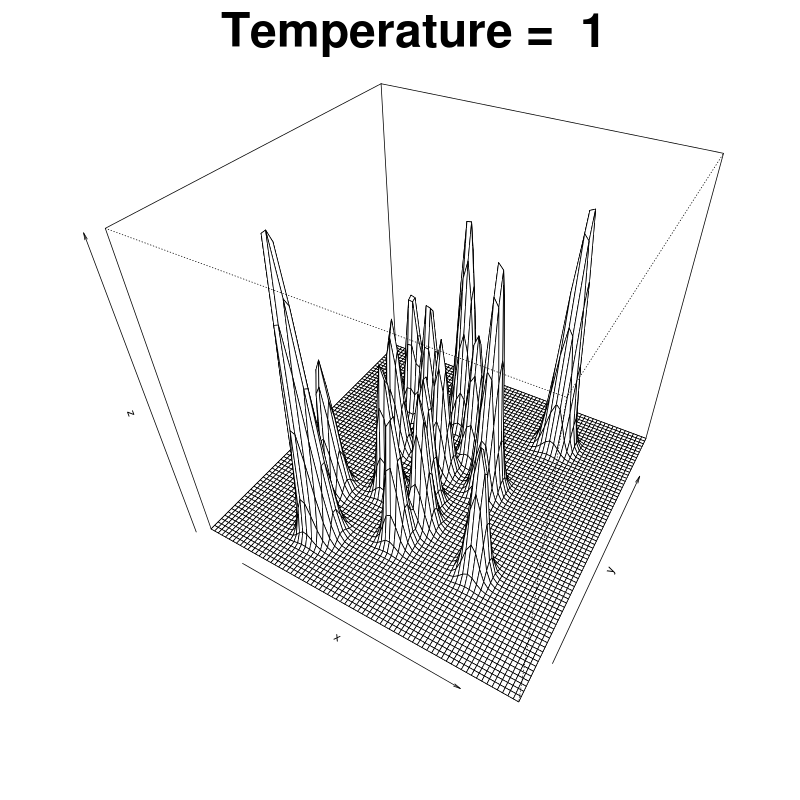
\includegraphics[width=1\textwidth]{img/Liang_perspective.png} 
      \end{minipage}
      & 
      {\small \begin{minipage}{0.75\linewidth}
        \bi 
          \item{ Let $\pi$ be a mixture of normal distributions
            \begin{equation*}
              \pi(x) = 
              \sum_{i=1}^{20} \frac{\omega_i}{ \sigma_i \sqrt{2 \pi} } \exp \Big( -\frac{(x - \mu_i)^\tran (x - \mu_i)}{2 \sigma_i^2} \Big)  
            \end{equation*} 
            where $\sigma_i$ are standard deviations, $\omega_i$ are weights, and $\mu_i$ are means \citep{Baragatti} 
          }
          \item{Some of the peaks mingle together to form bigger ones}
        \ei  
      \end{minipage}}
    \end{tabular}
  \end{center}

  \begin{center}
    \begin{tabular}[t]{cc}
      {\small \begin{minipage}{0.75\linewidth}
        \bi 
          \item{ 
            \GMH\, draws sample points from only two modes that are not far away from the starting points drawn at random from the region of the suspected probability concentration   
          }
          \item{
            Estimates of probabilities and moments are totally fallacious
          }
        \ei  
      \end{minipage}}
      &
      \begin{minipage}{0.25\linewidth}
        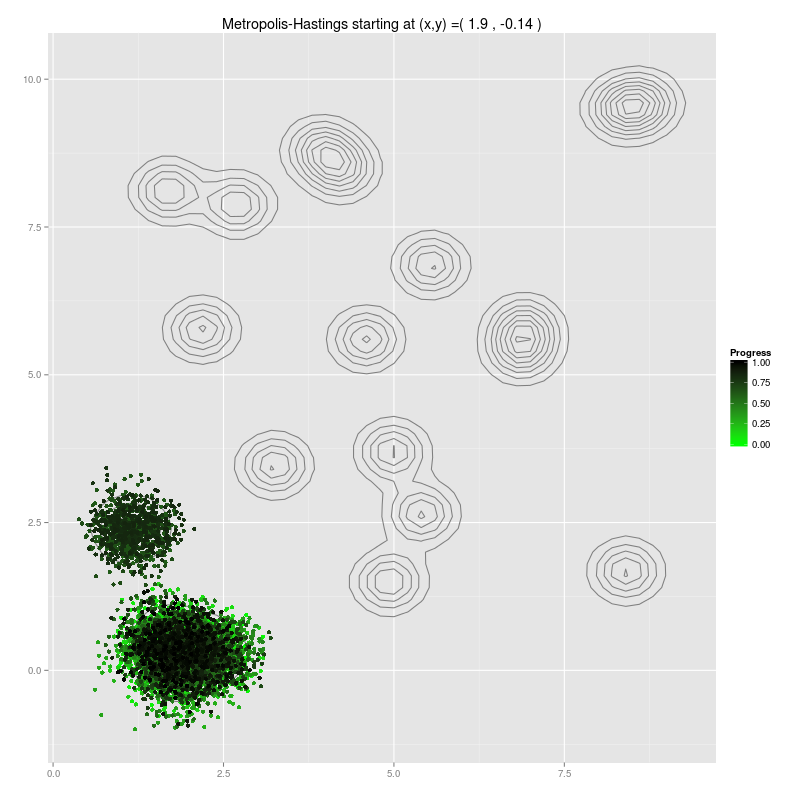
\includegraphics[width=.75\textwidth]{img/MH_simululation_10000_steps.png}
      \end{minipage} 
    \end{tabular}
  \end{center}
}

\coordinate (placeForQuestion) at ($(currenty)$);

%%%%%%%%%%%%%%%%%%%%%%%%%%%%%%%%%%%%%%%%%%%%%%%%%%%%%%%%%%%%%%%%%%%%%%%%%%%%%%%%%%%%%%%%%%%%%%%

\blocknode[($(currenty)-(0,2.5)$)]{Parallel Tempering a.k.a. Replica Monte Carlo}{   
  \bi
    \item{Foundations of \PT\, laid by \citet{RobertSwendsen}}
    \item{Generate several chains $X = [X_1, \dots, X_\llll]$} and consists of two phases
    \begin{phase}
      \item{ Drawing a point $\tilde{X}_l$ from $\pi^{\beta_l}$, where $1 = \beta_1 > \dots > \beta_\llll > 0$ are called inverse temperatures (note that first coordinate corresponds to our initial problem) \label{phaseOne} }
      \item{ Swaping some  of $\tilde{X}$ coordinates at random: the \textsc{Swap Strategy} \label{phaseTwo}}
    \end{phase}
    \item{ \ref{phaseOne} mitigates the impact of multimodiality enlarging the probability of accepting steps from regions which the \GMH\, would judge unlikely to draw from}
    \item{ \ref{phaseTwo} allows the passing of information from different chains: otherwise they would operate independently and first chain would gain nothing from other coordinates}
  \ei  
}

%%%%%%%%%%%%%%%%%%%%%%%%%%%%%%%%%%%%%%%%%%%%%%%%%%%%%%%%%%%%%%%%%%%%%%%%%%%%%%%%%%%%%%%%%%%%%%%


\plainblock[-5]{($(placeForQuestion)+(0,3.1)$)}{30}{?`Question?} %
{
  \vspace{0.3cm}\\
  How can we enhance mixing so that the \textsc{State Space} is better searched for probability clusters? 
}

%%%%%%%%%%%%%%%%%%%%%%%%%%%%%%%%%%%%%%%%%%%%%%%%%%%%%%%%%%%%%%%%%%%%%%%%%%%%%%%%%%%%%%%%%%%%%%%%%%%%%%%%%%%%%%%%%%%%%%%%%%%%%%%%%%%%%%%%%%%%%%%%%%%%%%%%%%%%%%%%%%%%%%%%%%%%%%%%%%%%%%%%%%%%%%

\startsecondcolumn
\blocknode{Parallel Tempering at work}
{
 \begin{tabular}[h]{cc}
    \begin{minipage}{0.5\linewidth}
      \bi
        \item{\small More tempered chains are at ease when passing from one mode to another\dots }
      \ei
      \centerline{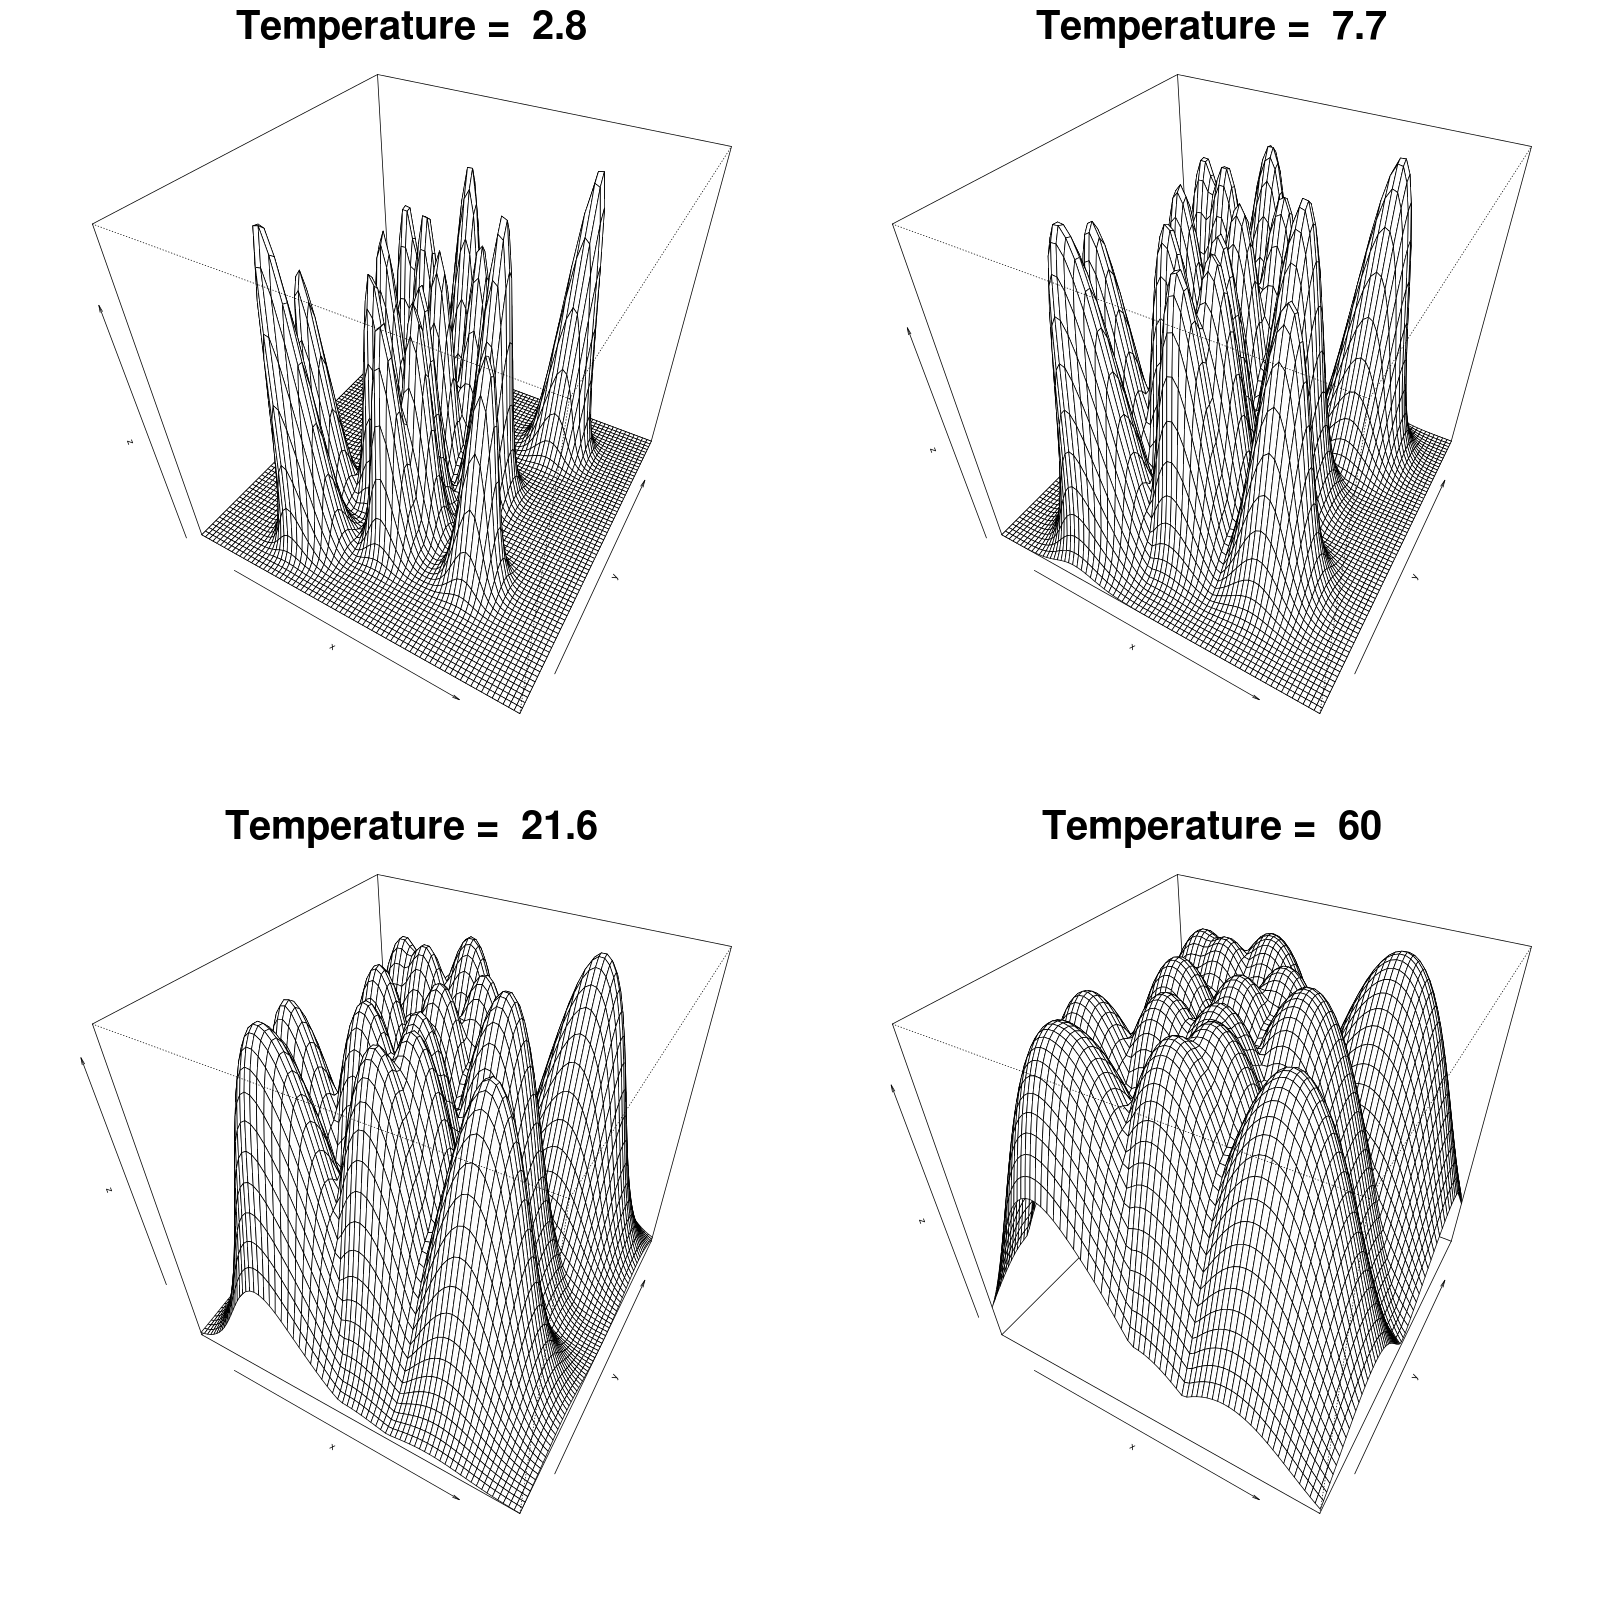
\includegraphics[width=.9\linewidth]{img/Liang_perspectives.png}}
    \end{minipage}
    &
    \begin{minipage}{0.5\linewidth}
      \bi
        \item{\small \dots and \ref{phaseTwo} assures that the base temperature chain explores more modes }
      \ei
      \centerline{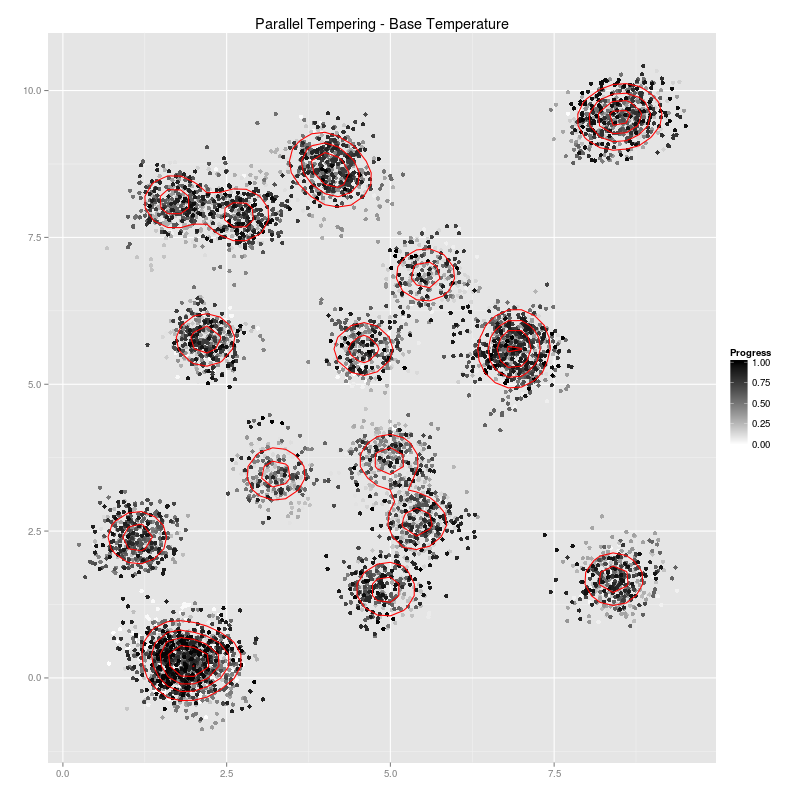
\includegraphics[width=.9\linewidth]{img/PT_simululation_base_temperature_10000_steps_1.png}}
    \end{minipage}
  \end{tabular}  
}


%%%%%%%%%%%%%%%%%%%%%%%%%%%%%%%%%%%%%%%%%%%%%%%%%%%%%%%%%%%%%%%%%%%%%%%%%%%%%%%%%%%%%%%%%%%%%%

\blocknode{Different Swap Strategies}
{ \small
  \bi
    \item In \ref{phaseTwo} one can implement a multitude of \textsc{Swap Strategies}
    \item Suppose that $\tilde{X}^{[k]} = x$. Then the distribution on the indices can be described as $p(i,j|x)$. We explored the following strategies ($\propto$ denotes proportionality and $\wedge$ - the minimum) 
  \ei

  \begin{tabular}[h]{cc}
    \begin{minipage}{0.3\linewidth}
      $$ p(i,j|x) \propto 
          \frac{\pi (x_j)}{\pi( x_i )} \wedge \frac{\pi (x_i)}{\pi( x_j )} $$
    \end{minipage}
    &
    \begin{minipage}{0.6\linewidth}
      {\small
        \textsc{Strategy} 1 promotes swaps between coordinates or relatively the same level, i.e. $\pi (x_j) \approx \pi (x_i)$
      }
    \end{minipage}
  \end{tabular}
  \begin{tabular}[h]{cc}
    \begin{minipage}{0.6\linewidth}
      {\small
        \textsc{Strategy} 2 breaks the symmetry of the previous one, giving more attention to swaps into regions of higher probability
      }
    \end{minipage}
    &
    \begin{minipage}{0.3\linewidth}
      $$ p(i,j|x) \propto 
          \frac{\pi (x_j)}{\pi (x_i)} \wedge 1 $$
    \end{minipage}
  \end{tabular}
  \begin{tabular}[h]{cc}
    \begin{minipage}{0.35\linewidth}
      $$ 
        p(i,j|x) \propto 
        \Big( \frac{\pi (x_j)}{\pi( x_i )} \wedge 
        \frac{\pi ( x_i)}{\pi( x_j )} \Big)^{\beta_i - \beta_j}  
      $$
    \end{minipage}
    &
    \begin{minipage}{0.55\linewidth}
      {\small
        \textsc{Strategy} 3 softens the requirement that $\pi(x_j) \approx \pi (x_i)$ for similarly tempered coordinates, i.e. where $\beta_i - \beta_j \approx 0$: swaps between adjacent chains get more probable
      }
    \end{minipage}
  \end{tabular}
  \begin{tabular}[h]{cc}
    \begin{minipage}{0.6\linewidth}
      {\small
        \textsc{Strategy} 4 generalises the last one favouring more distant choices: $\rho$ might any metric ({\it e.g.} euclidean)
      }
    \end{minipage}
    &
    \begin{minipage}{0.3\linewidth}
      $$ p(i,j|x) \propto \Big( \frac{\pi (x_j)}{\pi( x_i )} \wedge \frac{\pi (x_i)}{\pi( x_j )} \Big)^\frac{\beta_i - \beta_j}{1 + \rho(x_i, x_j)} $$
    \end{minipage}
  \end{tabular}
  
  \bi
    \item{All the above strategies explicitly refer to values of $\pi$ in points drawn in \ref{phaseOne} making the draws computationally cheap}
    \item{\textsc{Strategies} 5 and 6 are independent of evaluations of $\pi$ giving equal probability to all possible and all neighbouring swaps respectively}
    \item{Beneath we represent results obtained by all the strategies when trying to approximate the values of different modes: they should be equal roughly to $0.05$, $\pi$ being a mixture of $20$ equally probable normal distributions. Result were obtained after $240$ runs of \PT\, with $2500$ steps of burn-in and $7500$ steps of simulations}  
  \ei

  \centerline{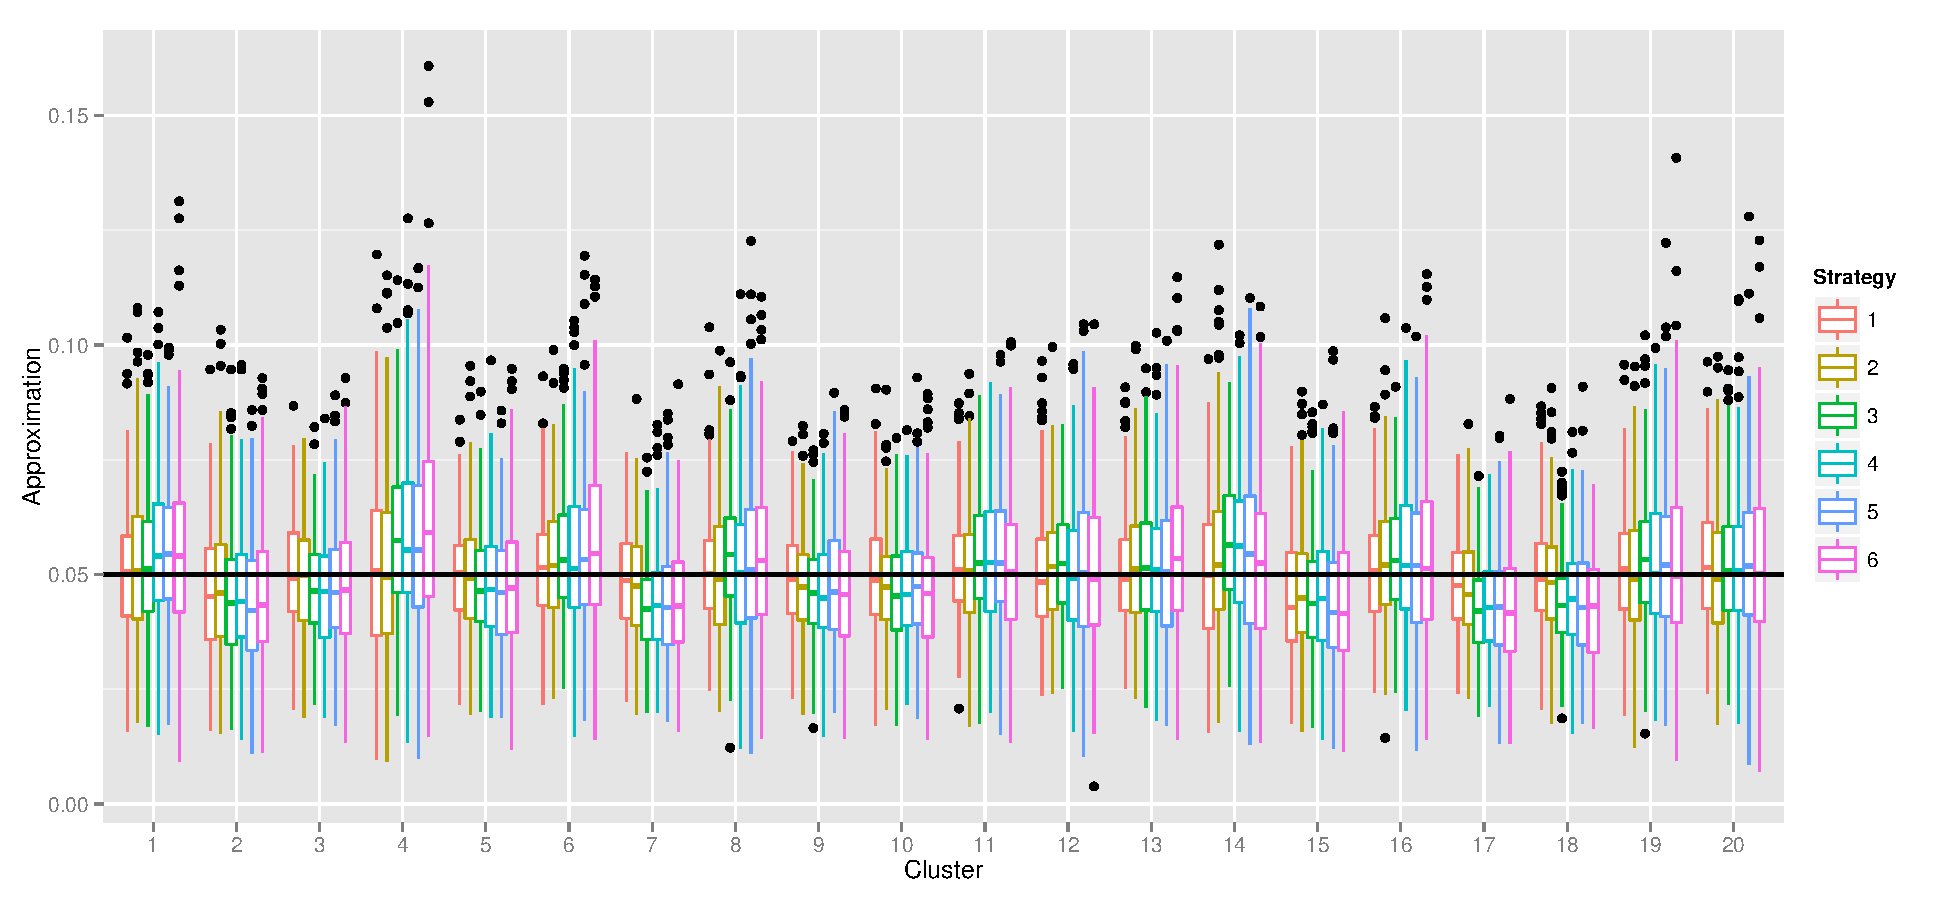
\includegraphics[width=1\linewidth]{img/comparison.pdf}} 
}

\coordinate (placeForAdvertisement) at ($(currenty)$);

%%%%%%%%%%%%%%%%%%%%%%%%%%%%%%%%%%%%%%%%%%%%%%%%%%%%%%%%%%%%%%%%%%%%%%%%%%%%%%%%%%%%%%%%%%%%%%%%%%%%%%%%%%%%%%%%%%%%%%%%%%%%%%%%%%%%%%%%%%%%%%%%%%%%%%%%%%%%%%%%%%%%%%%%%%%%%%%%%%%%%%%%%%%%%%

%\startthirdcolumn

\blocknode[($(currenty)-(0,14)$)]{References}{
  \bibliographystyle{bibliography/eccaNoNotes}
  \tiny{ 
    \bibliography{bibliography/references}
  }
}

\plainblock[5]{($(placeForAdvertisement)+(0,3.1)$)}{34.5}{!`Good Software Available Soon!} %
{
  %\vspace{0.3cm}\\
  \bi
    \item{ An \textsc{R} package, under the working name of \textsc{StochasticSimulations}, will be soon available for widespread use for free}
    \item{ Among its features}
    \bi
      \item{ Division of the simulations into modules: \textsc{Algorithm}, \textsc{State Space}, \textsc{Target Measure} will provide a logic for the implementation of different models}
      \item{ Implementation of the most common choices for \textsc{State Space}: $\real^\mathrm{S}$ and \textsc{Discrete} state space}
      \item{ Implementation of the \GMH\, and \PT\,algorithms with the above-mentioned \textsc{Strategies}}
      \item{ \textsc{GGPLOT} 2 based visualisations }
    \ei
    \item{ \dots and much, much more: stay tuned!}
  \ei  
}


\end{tikzpicture}


\end{document}



%%%%%%%%%%%%%%%%%%%%%%%%%%%%%%%%%%%%%%%%%%%%%%%%%%%%%%%%%%%%%%%%%%%%%%%%%%%%%%%%%%%%%%%%%%%%%%%%%%%%%%%%%%%%%%%%%%%%%%%%%%%%%%%%%%%%%%%%%%%%%%%%%%%%%%%%%%%%%%%%%%%%%%%%%%%%%%%%%%%%%%%%%%%%%%%%%%%%%%%%%%%%%%%%%%%%%%%%%%%%%%%%%%%%%%%%%%%%%%%%%%%%%%%%%%%%%%%%%%%%%%%%%%%%%%%%%%%%%%%%%%%%%%%%%%%%%%%%%%%%%%%%%%%%%%%%%%%%%%%%%%%%%%%%%%%%%%%%%%%%%%%%%%%%%%%%%%%%%%%%%%%%%%%%%%%%%%%%%%%%%%%%%%%%%%%%%%%%%%%%%%%%%%%%%%%%%%%%%%%%%%%%%%%%%%%%%%%%%%%%%%%%%%%%%%%%%%%%%%%%%%%%%%%%%%%%%%%%%%%%%%%%%%%%%%%%%%%%

% \plainblock[5]{($(currenty)+(-5,0)$)}{26}{Multimodial Example} %
% {
%   \vspace{0.3cm}\\
%   Consider $\pi$ given by density $f$ that is a mixture of normal distributions
%   \begin{equation*}
%     f(x) = 
%     \sum_{i=1}^{20} \frac{\omega}{ \sigma \sqrt{2 \pi} } \exp \Big( -\frac{(x - \mu_i)^\tran (x - \mu_i)}{2 \sigma^2} \Big),  
%   \end{equation*}
%   s.t. $\sigma = 0.1$, $\omega = 0.05 $, with means 

%   {
%     \centering
%     \tiny{
%       \begin{tabular}{rrrrrrrrrrrrrrrrrrrr}
%         \hline
%       $\mu_1$ & $\mu_2$ & $\mu_3$ & $\mu_4$ & $\mu_5$ & $\mu_6$ & $\mu_7$ & $\mu_8$ & $\mu_9$ & $\mu_{10}$ & $\mu_{11}$ & $\mu_{12}$ & $\mu_{13}$ & $\mu_{14}$ & $\mu_{15}$ & $\mu_{16}$ & $\mu_{17}$ & $\mu_{18}$ & $\mu_{19}$ & $\mu_{20}$ \\ 
%         \hline
%       2.18 & 8.67 & 4.24 & 8.41 & 3.93 & 3.25 & 1.70 & 4.59 & 6.91 & 6.87 & 5.41 & 2.70 & 4.98 & 1.14 & 8.33 & 4.93 & 1.83 & 2.26 & 5.54 & 1.69\\ 
%         5.76 & 9.59 & 8.48 & 1.68 & 8.82 & 3.47 & 0.50 & 5.60 & 5.81 & 5.40 & 2.65 & 7.88 & 3.70 & 2.39 & 9.50 & 1.50 & 0.09 & 0.31 & 6.86 & 8.11\\ 
%          \hline
%       \end{tabular}
%     }
%   }
% }

%%%%%%%%%%%%%%%%%%%%%%%%%%%%%%%%%%%%%%%%%%%%%%%%%%%%%%%%%%%%%%%%%%%%%%%%%%%%%%%%%%%%%%%%%%%%%%%
% \blocknode[($(currenty)-(0,15)$)]{Parallel Tempering}{   
% Hello.
% }

% \blocknode[($(currenty)-(0,15)$)]{Fallacious Inferences}{   
%   \begin{tikzfigure}
%     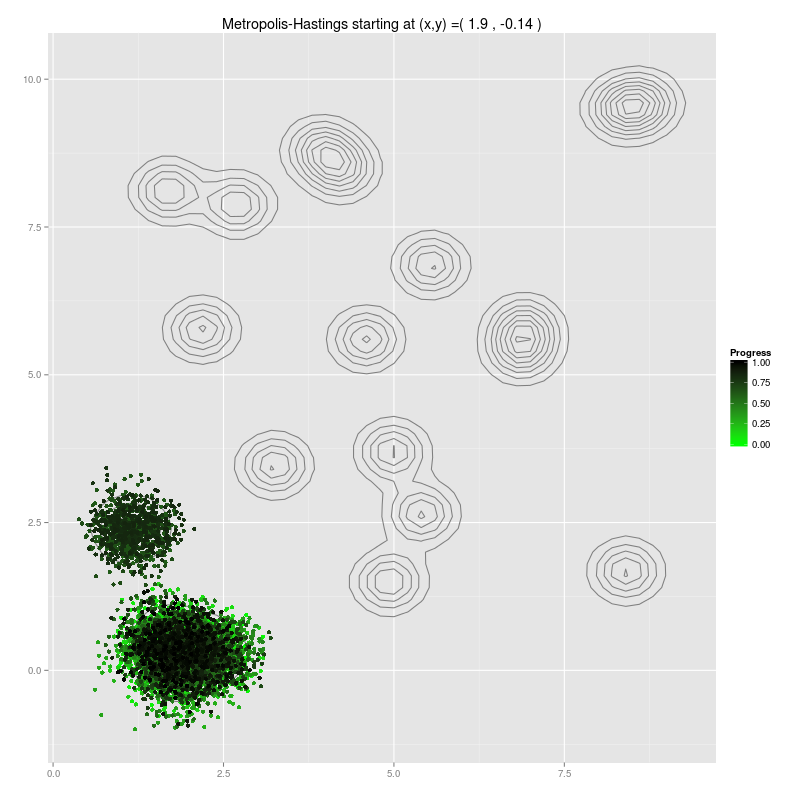
\includegraphics[scale=.2]{img/MH_simululation_10000_steps.png}
%   \end{tikzfigure}  
% }

% \blocknode{Picture}{
%   \begin{tikzfigure}[Metropolis Hastings]
    % 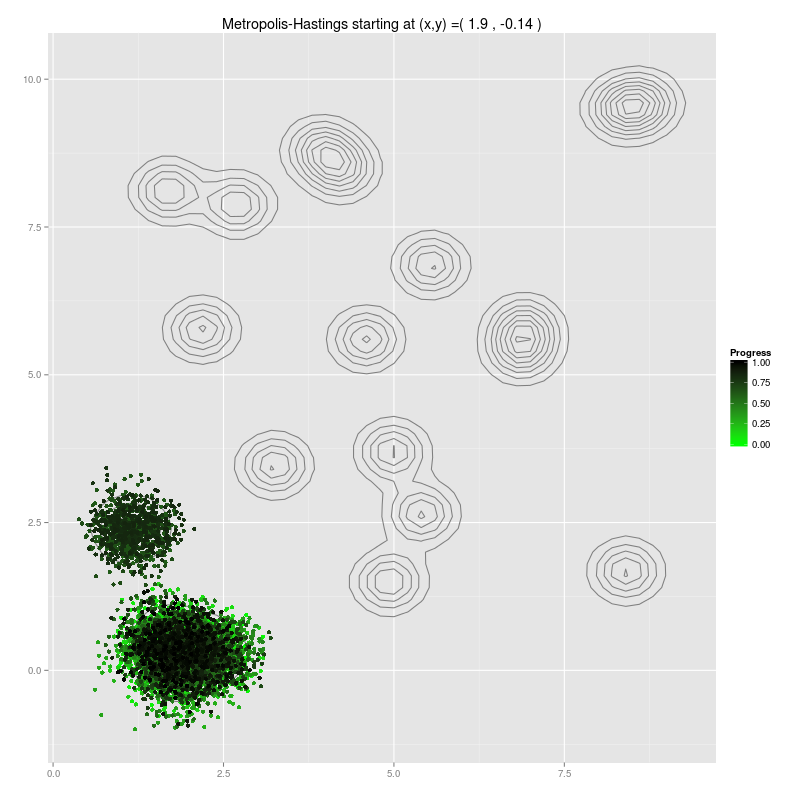
\includegraphics[scale=.3]{img/MH_simululation_10000_steps.png}
%   \end{tikzfigure}
% } 


% \bi
  %   \item In \ref{phaseTwo} one can implement a multitude of \textsc{Swap Strategies}
  %   \item Suppose that $\tilde{X}^{[k]} = x$. Then the distribution on the indices can be described as $p(i,j|x)$. We explored the following strategies ($\propto$ denotes proportionality and $\wedge$ - the minimum) 
  %   \begin{strategy}
      
  %     \item{ 
  %       $$
  %         p(i,j|x) \propto 
  %         \frac{\pi (x_j)}{\pi( x_i )} \wedge \frac{\pi (x_i)}{\pi( x_j )} 
  %       $$ 
    
  %       This strategy assures that the more probable swaps will occur between coordinates that are relatively the same, i.e. $\pi (x_j) \approx \pi (x_i)$
  %     }  
    
  %     \item{ 
  %       $$
  %         p(i,j|x) \propto 
  %         \frac{\pi (x_j)}{\pi (x_i)} \wedge 1 
  %       $$
    
  %       This strategy breaks the symmetry of the previous one. This strategy gives more attention to swaps into regions of higher probability
  %     }
  
  %     \item{ 
  %       $$
          % p(i,j|x) \propto 
          % \Big( \frac{\pi (x_j)}{\pi( x_i )} \wedge 
          % \frac{\pi ( x_i)}{\pi( x_j )} \Big)^{\beta_i - \beta_j} 
  %       $$ 

        % This strategy permits us to soften a bit the requirement that $\pi(x_j) \approx \pi (x_i)$. This effect is strengthened for coordinates that are similarly tempered, i.e. where $\beta_i - \beta_j \approx 0$, making swaps between adjacent chains more probable
  %     }

  %     \item{ 
  %       $$
  %         p(i,j|x) \propto \Big( \frac{\pi (x_j)}{\pi( x_i )} \wedge \frac{\pi (x_i)}{\pi( x_j )} \Big)^\frac{\beta_i - \beta_j}{1 + \rho(x_i, x_j)} 
  %       $$
 
  %       This strategy generalises the last one - $\rho$ might be any distance between coordinates ({\it e.g.} euclidean), so as to favour more distant choices and better mixing
  %     }  
  %   \end{strategy}

  % \blocknode{Good Software Available Soon}{
%   \bi
%     \item{ An \textsc{R} package, under the working name of \textsc{StochasticSimulations}, will be soon available for widespread use for free}
%     \item{ Among its features}
%     \bi
%       \item{ Division of the simulations into modules: \textsc{Algorithm}, \textsc{State Space}, \textsc{Target Measure} will provide a logic for the implementation of different models}
%       \item{ Implementation of the most common choices for \textsc{State Space}: $\real^\mathrm{S}$ and \textsc{Discrete} state space}
%       \item{ Implementation of the \GMH\, and \PT\,algorithms with the above-mentioned \textsc{Strategies}}
%       \item{ \textsc{GGPLOT} 2 based visualisations }
%     \ei
%     \item{ \dots and much, much more: stay tuned!}
%   \ei  
% }

% \blocknode{References}{
%   \bibliographystyle{bibliography/eccaNoNotes}
%   \tiny{ 
%     \bibliography{bibliography/references}
%   }
% }
